Let $\boldsymbol{A}$ be a $2 \times 2$ matrix

\begin{align*}
    \boldsymbol{A} = \begin{bmatrix}
        x_1 & x_2 \\
        y_1 & y_2
    \end{bmatrix}
\end{align*}

Show that the magnitude of $\det(\boldsymbol{A})$ is equal to the area of the parallelogram formed by the column vectors of the matrix $\boldsymbol{A}$.

\begin{solution}\ \\    \begin{center}
        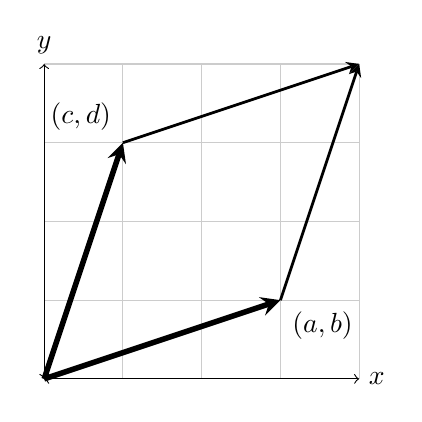
\begin{tikzpicture}
          \draw[thin,gray!40] (0,0) grid (4,4);
          \draw[<->] (0,0)--(4,0) node[right]{$x$};
          \draw[<->] (0,0)--(0,4) node[above]{$y$};
          \draw[line width=2pt,black,-stealth](0,0)--(3,1) node[anchor=north west]{$(a, b)$};
          \draw[line width=2pt,black,-stealth](0,0)--(1,3) node[anchor=south east]{$(c, d)$};
          \draw[line width=1pt,black,-stealth](3,1)--(4,4);
          \draw[line width=1pt,black,-stealth](1,3)--(4,4);
        \end{tikzpicture}
    \end{center}

    \begin{align*}
        area &= \left(a + c\right)\left(b + d\right) - \left(2bc + 2\left(\frac{1}{2}ab\right) + 2\left(\frac{1}{2}cd\right)\right) \\
        area &= ab + ad + cb + cd - 2bc - ab - cd \\
        area &= ad - bc
    \end{align*}
\end{solution}
